\documentclass[12pt]{article}

\usepackage[utf8]{inputenc} 

\usepackage{graphicx} %to add images

\usepackage{hyperref} %to add references

\hypersetup{
    colorlinks=true,
    linkcolor=blue,
    filecolor=magenta,      
    urlcolor=cyan,
}

\begin{document}


%	TITLE PAGE


\begin{titlepage} 
	\newcommand{\HRule}{\rule{\linewidth}{0.5mm}} 
	
	\center 
	
	
	%	Headings
-
	
	\textsc{\LARGE Indian Institute Of Technology Kanpur}\\[1.5cm] % Main heading
	
	\textsc{\Large Assignment 5}\\[0.5cm] % Major heading such as project name
	
	\textsc{\Large CS253 - Software Development And Operations}\\[0.5cm] % Minor heading such as course title
	

	%	Title

	\HRule\\[0.4cm]
	
	{\huge\bfseries Three Khans of Bollywood}\\[0.4cm] % Title of your document
	
	\HRule\\[1.5cm]
	
	\large
			\textsc{Atur Gupta(190203)}\\
	
	
    \vfill\vfill\vfill % Position the date 3/4 down the remaining page
	
	{\large\today} % Date
	
	\vfill % Push the date up 1/4 of the remaining page
	
\end{titlepage}

%----------------------------------------------------------------------------------------

\section{Performance of each Khan at the Box Office}

\subsection{Salman Khan}

\subsubsection{Box Office Collection}

\begin{figure}[h]
    %\centering
    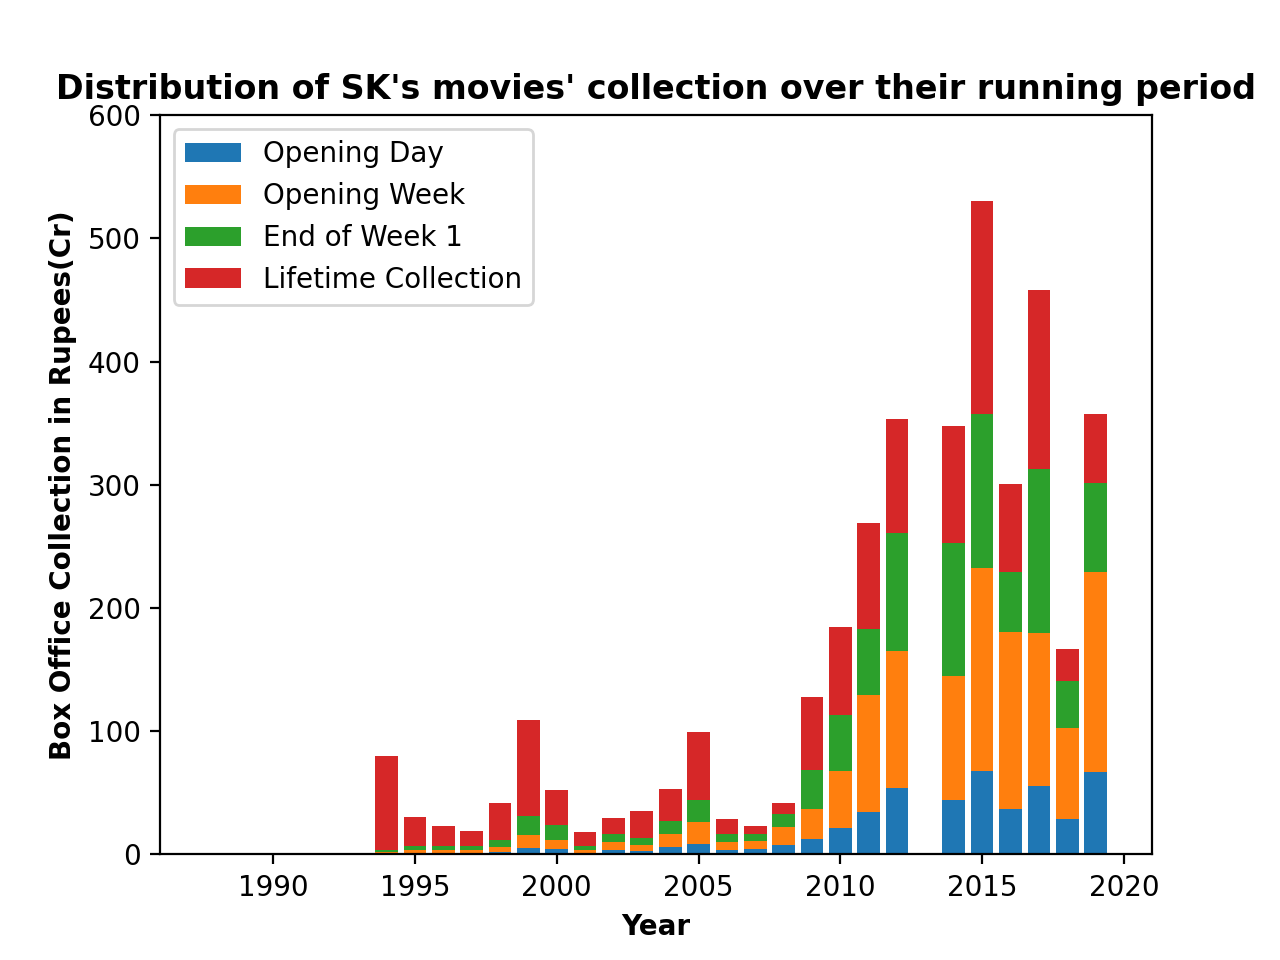
\includegraphics[width=12cm]{skstack.png}
    \caption{Salman Khan}
    \label{fig:BOC}
\end{figure}

Salman Khan is one of the best-performing actors at the box office in today's date. He has the biggest fanbase in India among all the actors as is evident from his above box office collection records, which clearly show his growth at the Indian Cinema in terms of movie revenues. 
\newline
\newline
We can see that since the start of his career from around 1992 for the next 10-15 years, only a handful of his movies went to earn around 100 Cr. But since 2009, all of his movies not only pass the 100 Cr threshold but most of his films now make a lifetime collection of over 200-300 Crores now. This humongous change is also a very strong indicator of the fact that Cinematic Industry has bloomed outstandingly in the past decade. 

\subsubsection{Movies' Verdicts}

\begin{figure}[h]
    %\centering
    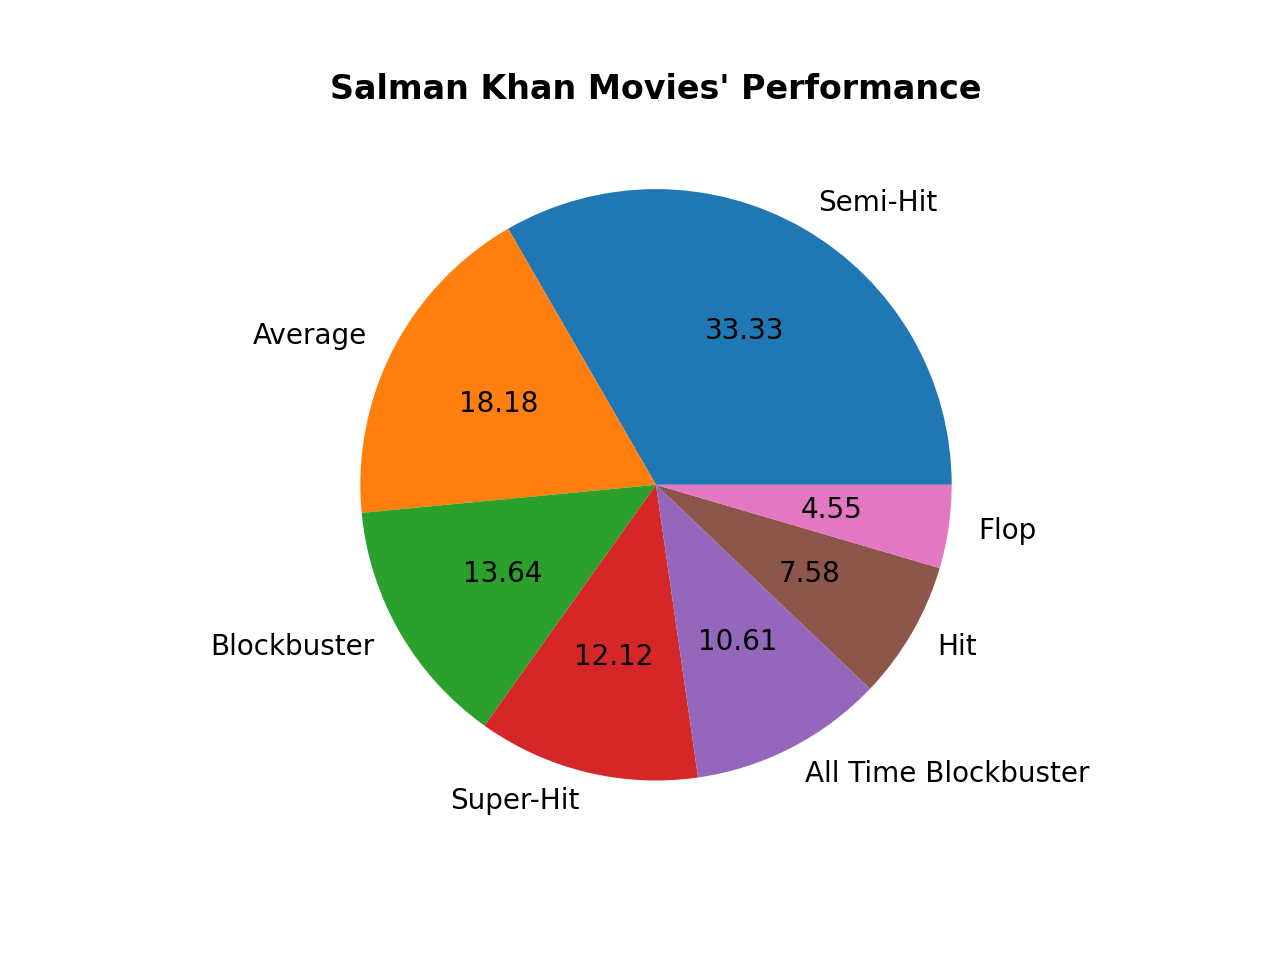
\includegraphics[width=12cm]{skpie.png}
    \caption{Salman Khan}
    \label{fig:Verdict}
\end{figure}

It is jaw-dropping how less number of flops(only $5\%$) Salman Khan has made. Most of his movies are semi-hit which is a feat in itself.
Also, every one of his three movies is a super-hit or even better. 
\clearpage

\subsection{Shah Rukh Khan}

\subsubsection{Box Office Collection}

\begin{figure}[h]
    %\centering
    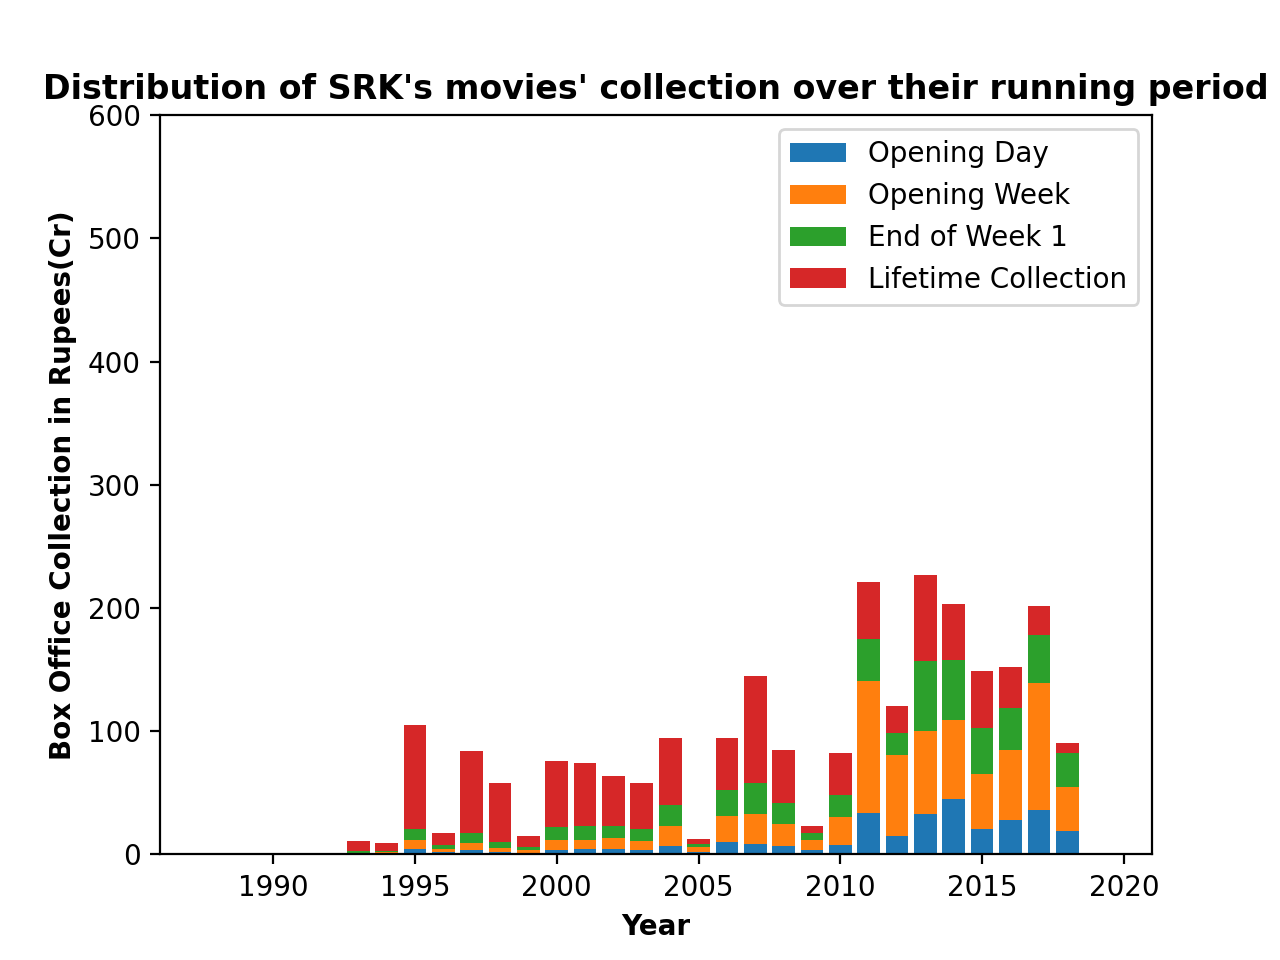
\includegraphics[width=12cm]{srkstack.png}
    \caption{Shah Rukh Khan}
    \label{fig:BOC}
\end{figure}

Looking at the above plot, one can straight away understand why SRK was given the name King Khan. He also started his career around 1992-93 and just look how great he did in his first 10 years of Bollywood. Almost every year box office collection touched 70-80 Crores and we're talking 15-20 years in past, when cinema was still a luxury for most and one rupee's value was much higher. 
\newline
\newline
Though it is also clear that the graph has its peak at around 2012 and since then it's mostly been on decline, which makes sense since his last movies have not done so well to his name. 

\clearpage

\subsubsection{Movies' Verdicts}

\begin{figure}[h]
    %\centering
    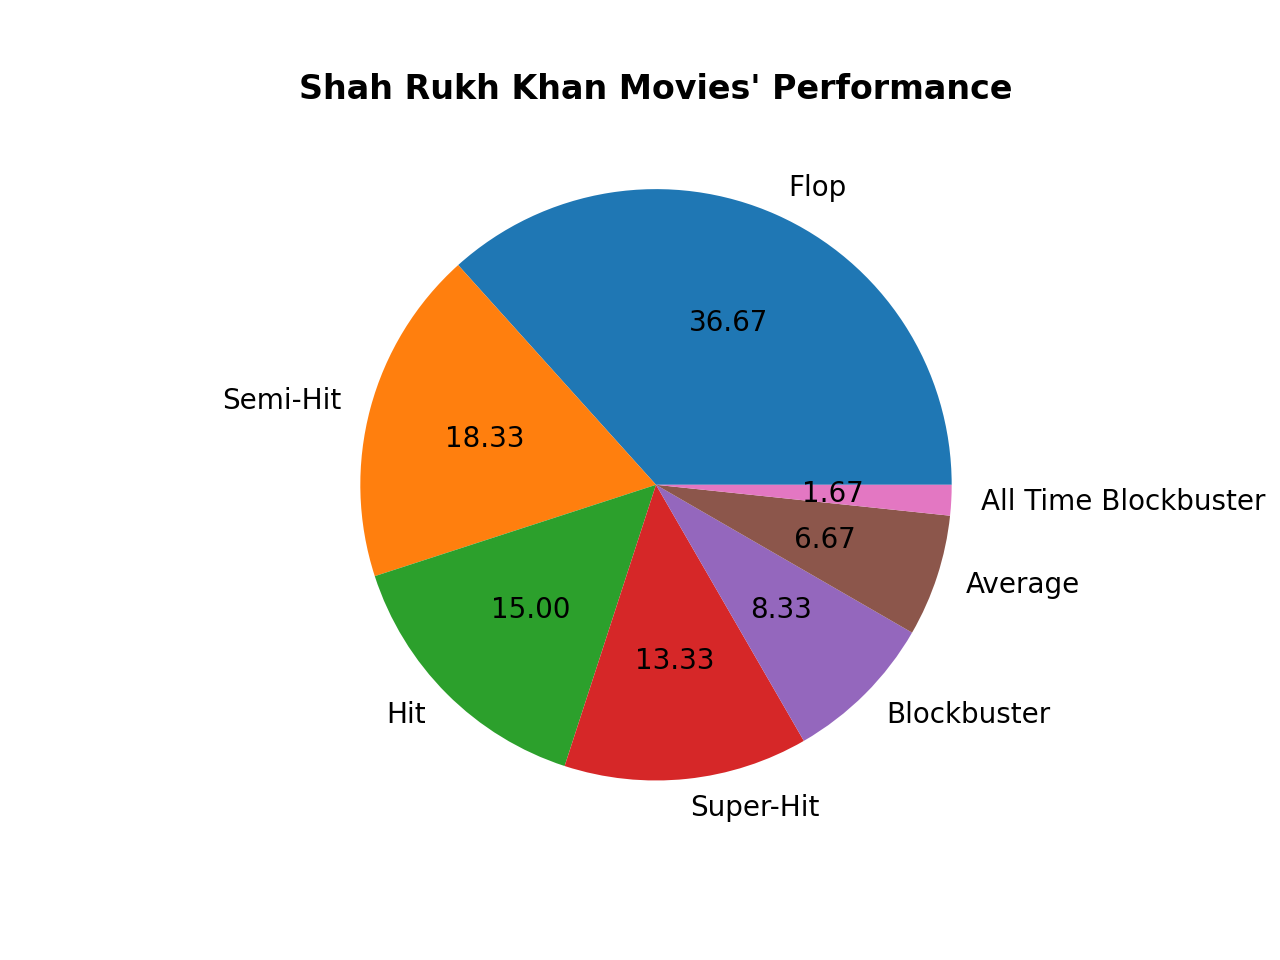
\includegraphics[width=12cm]{srkpie.png}
    \caption{Shah Rukh Khan}
    \label{fig:Verdict}
\end{figure}

One-third of the SRK's movies are considered flops, and if we look at the data, it's clear that this results from the fact that his performance has been poor for the better part of the past decade. 
\newline
\newline
He is counted among the actors having the longest streak of giving hit movies but his performance and choice of selection of movies in the last some years has all but brought down his name. 
\clearpage

\subsection{Aamir Khan}

\subsubsection{Box Office Collection}

\begin{figure}[h]
    %\centering
    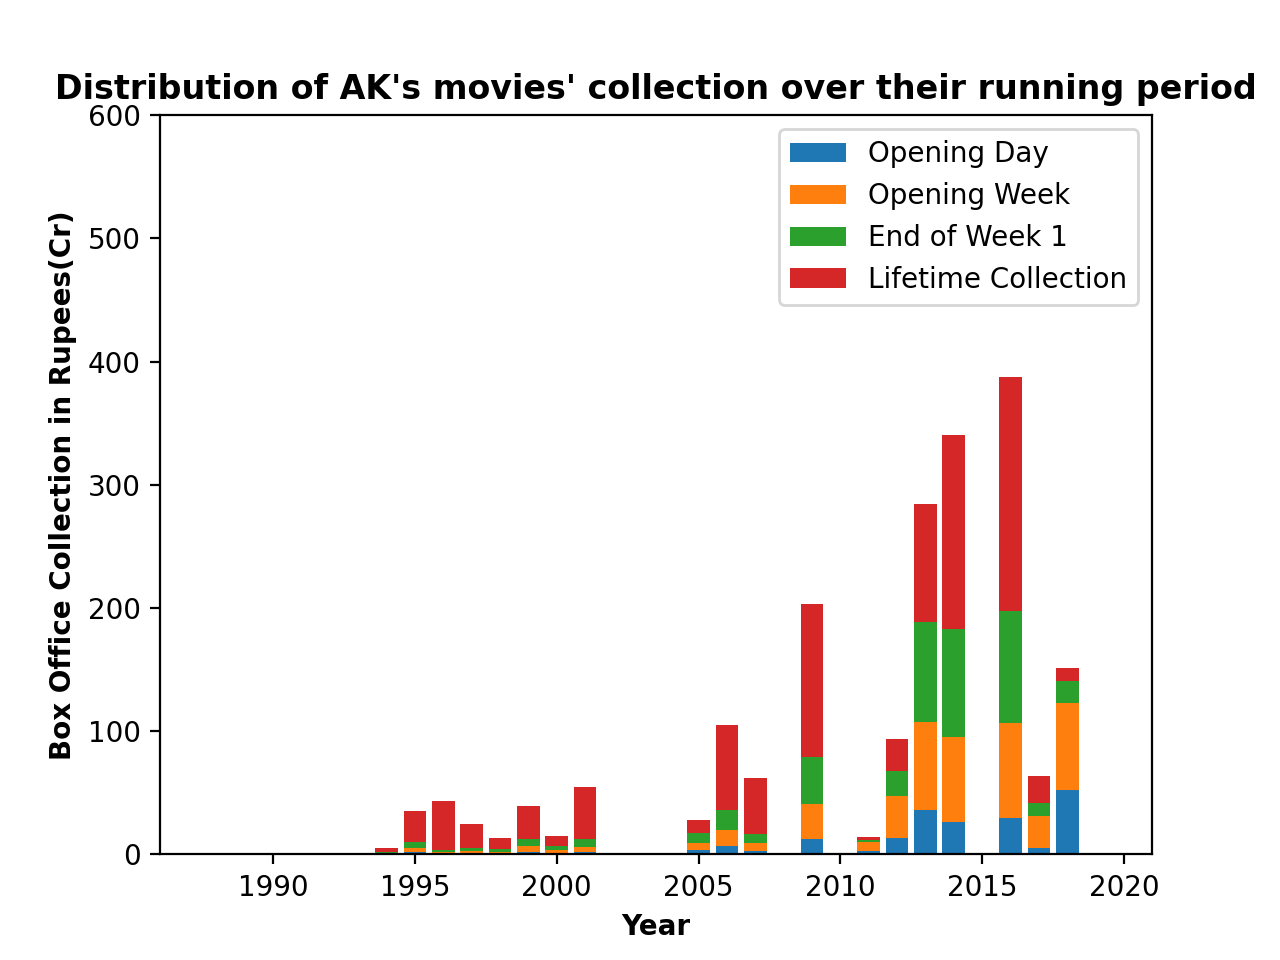
\includegraphics[width=12cm]{akstack.png}
    \caption{Aamir Khan}
    \label{fig:BOC}
\end{figure}

 Aamir Khan doesn't do a whole lot of movies. We can even see some gap years in between. But at the same time it's also clear that his movies perform very good at the box office, shown by 4 bars above 200 Cr. Giving evidence to the saying that he is a perfectionist and tries to make his movie a perfection even if it means doing one or two less movies a year.
\newline
\newline
Peak at 2009 and 2014 must be obviously due to the my-all-time-favourites 3 Idiots and PK respectively.

\clearpage

\subsubsection{Movies' Verdicts}

\begin{figure}[h]
    %\centering
    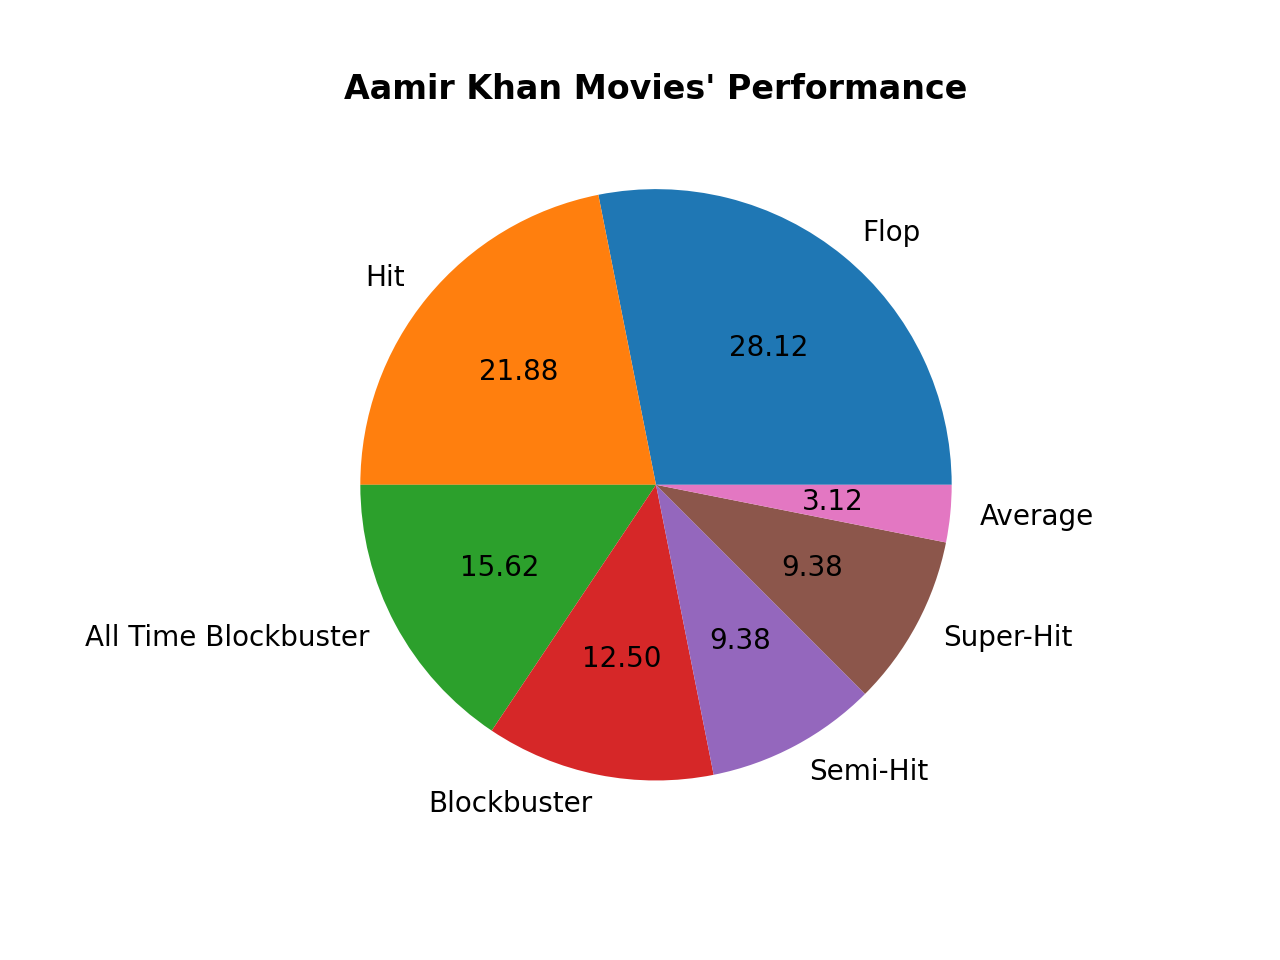
\includegraphics[width=12cm]{akpie.png}
    \caption{Aamir Khan}
    \label{fig:Verdict}
\end{figure}

One amazing thing that we observe from the above pie chart is that the total number of Average and Semi-Hit movies is very few in number, which tells us that either his movies mostly go Hit or Flops, very rarely average. Which in turn then tells us that he experiments with his choice of selection of movies and challenges himself with them. This fact everybody knows to be true and it's great that we can infer that from this data.  
\clearpage

\section{Comparison between the Three Khans}

\subsection{Box Office Revenue}
\begin{figure}[h]
    %\centering
    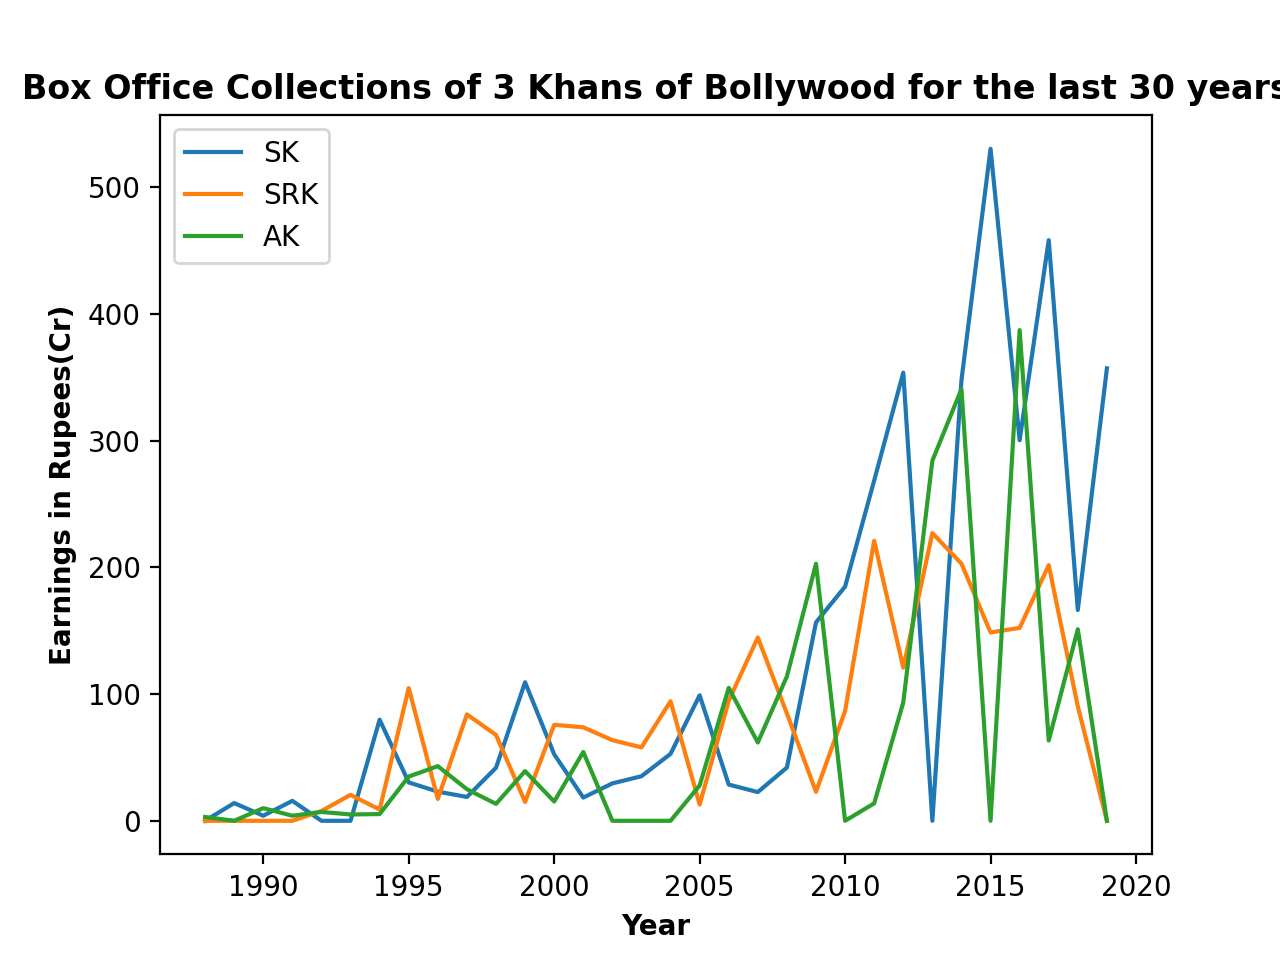
\includegraphics[width=12cm]{line.png}
    \caption{Line Plot}
    \label{fig:Verdict}
\end{figure}
As we also talked above, we see that from 1995 to around 2008, it could be said that SRK was performing the best among the 3 in terms of Collections. Here and there, we see Salman Khan coming up with a big hit but mostly it was SRK who had the upper hand over other 2. 
\newline
\newline
But from 2009 till present, we see a very drastic change and observe that SRK's movies' collections is the lowest by considerable amount. This reiterates the fact that we discussed above that the past decade just wasn't in SRK's favour. 
\newline
Salman Khan has done exceptionally well reaching different heights altogether, through the unflinching support of his loyal fans undoubtedly.  
\clearpage

\subsection{Movies' Verdicts}
\begin{figure}[h]
    %\centering
    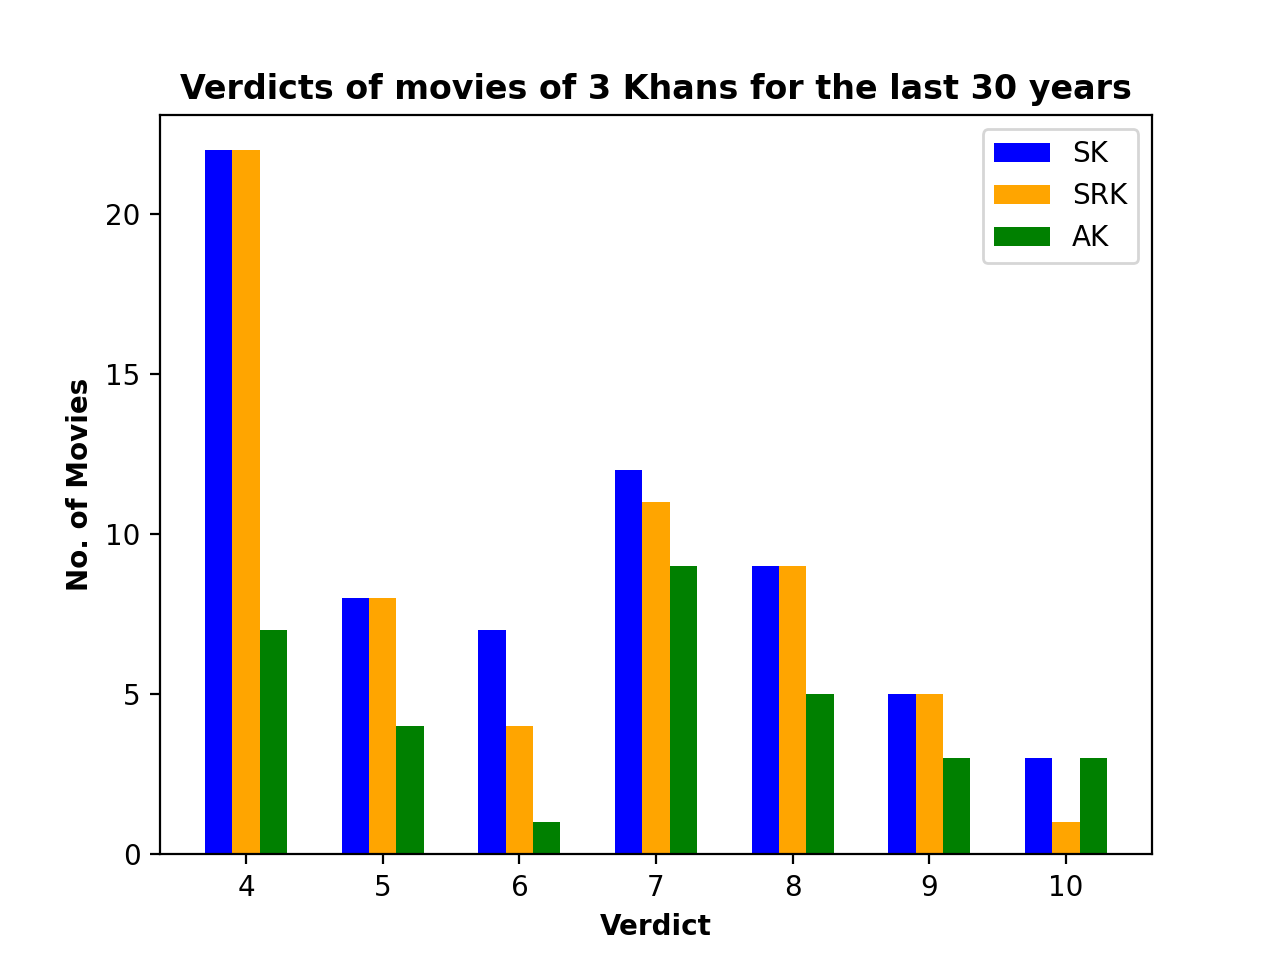
\includegraphics[width=12cm]{groupbar.png}
    \caption{Group Bar Plot}
    \label{fig:Verdict}
\end{figure}

[All Time Blockbuster = 10
    , Blockbuster = 9
    , Super-Hit = 8
    , Hit = 7
    , Semi-Hit = 6
    , Average = 5
    , Flop = 4]
    \newline
    \newline

There are 2 Noteworthy things here - First is that Aamir Khan has made quite less (almost half) number of movies as compared to the other two, while Salman Khan has made the most.
\newline
Second is that while Aamir Khan is a bit behind Salman Khan and Shah Rukh khan in terms of giving hits, he has given significantly less number of flops than the other two. 
\newline
This data again strengthens the fact that AK puts his all into his movies and does it for the art and not just for the money.  

\clearpage

\section{Correlation between earnings and verdict}

\begin{figure}[h]
    %\centering
    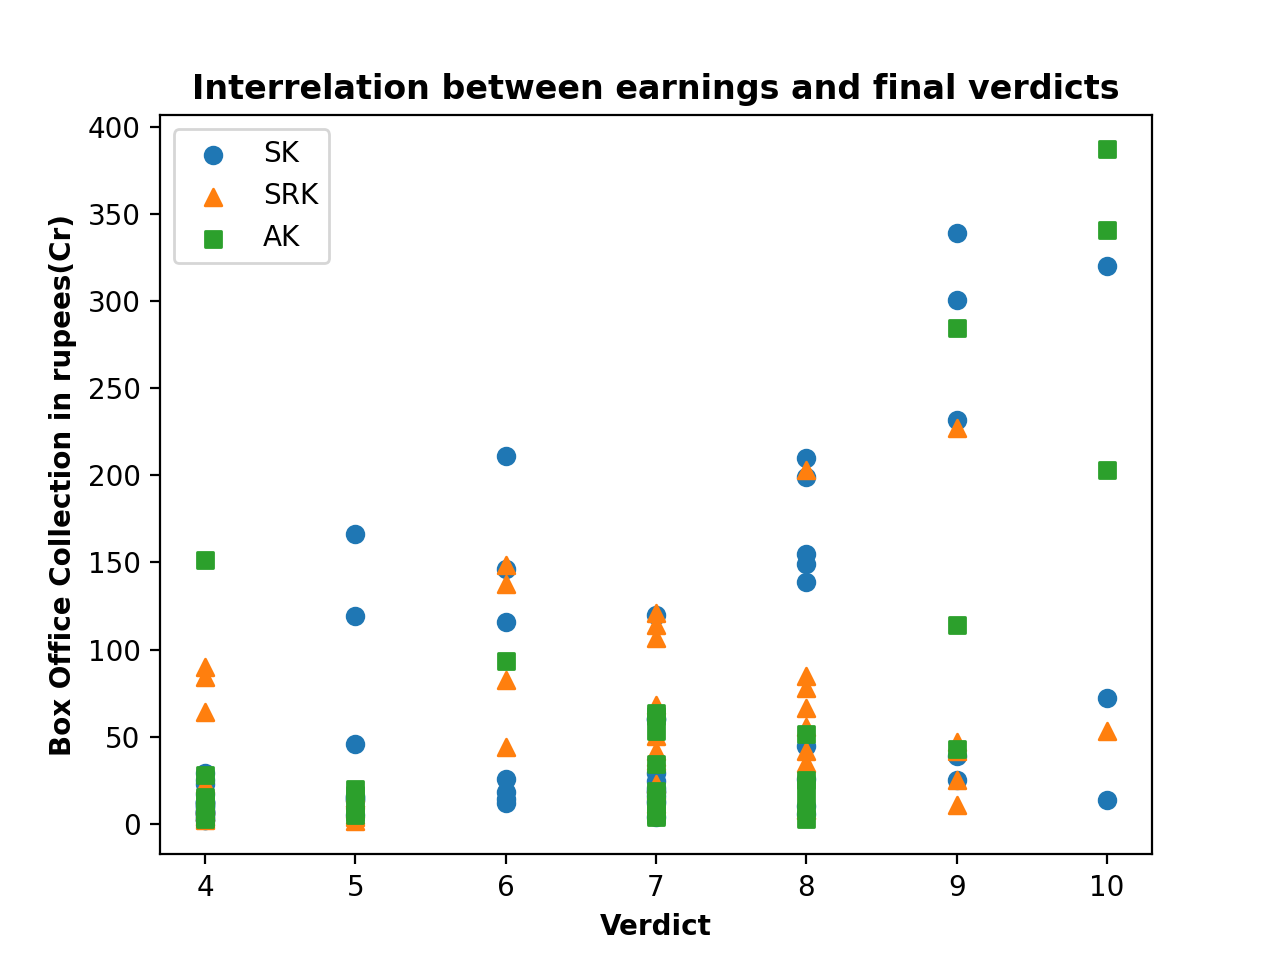
\includegraphics[width=12cm]{scatter.png}
    \caption{Scatter plot}
    \label{fig:Verdict}
\end{figure}

Now, this is an interesting graph. It reminds us of the very important fact that we can't say a film was a hit or a flop just by looking at the earnings of the film. We need to know about the budget, date of release and maybe some other extra resources put into the film too.
\newline
\newline
From the above chart, we see that if a movie has earned less than 200 Crores, It can be given any verdict from 4 to 9 with similar probability. A movie earning 50 Crore could be a Blockbuster and a movie earning a whopping 150 Crores could still be considered having an average performance at the box office.  
\newline
Though the movies earning more than 300 Crores are very likely to be Blockbusters, since as of today most movies in India don't have that kind of a budget and hence it's with a very high probability that that movie has made tons of profits at the Indian Box Office. 

\clearpage

\section{References}

All the data has been taken from the site \href{https://www.bollywoodhungama.com/}{Bollywoodhungama}. Links are given below - 

\begin{itemize}
    \item \href{https://www.bollywoodhungama.com/celebrity/shah-rukh-khan/box-office/#bh-micro-tab-content}{Shah Rukh Khan}
    
    \item \href{https://www.bollywoodhungama.com/celebrity/salman-khan/box-office/#bh-micro-tab-content}{Salman Khan}
    
    \item \href{https://www.bollywoodhungama.com/celebrity/aamir-khan/box-office/#bh-micro-tab-content}{Aamir Khan}
\end{itemize}





\end{document}

